% Options for packages loaded elsewhere
\PassOptionsToPackage{unicode}{hyperref}
\PassOptionsToPackage{hyphens}{url}
%
\documentclass[
]{book}
\usepackage{amsmath,amssymb}
\usepackage{iftex}
\ifPDFTeX
  \usepackage[T1]{fontenc}
  \usepackage[utf8]{inputenc}
  \usepackage{textcomp} % provide euro and other symbols
\else % if luatex or xetex
  \usepackage{unicode-math} % this also loads fontspec
  \defaultfontfeatures{Scale=MatchLowercase}
  \defaultfontfeatures[\rmfamily]{Ligatures=TeX,Scale=1}
\fi
\usepackage{lmodern}
\ifPDFTeX\else
  % xetex/luatex font selection
\fi
% Use upquote if available, for straight quotes in verbatim environments
\IfFileExists{upquote.sty}{\usepackage{upquote}}{}
\IfFileExists{microtype.sty}{% use microtype if available
  \usepackage[]{microtype}
  \UseMicrotypeSet[protrusion]{basicmath} % disable protrusion for tt fonts
}{}
\makeatletter
\@ifundefined{KOMAClassName}{% if non-KOMA class
  \IfFileExists{parskip.sty}{%
    \usepackage{parskip}
  }{% else
    \setlength{\parindent}{0pt}
    \setlength{\parskip}{6pt plus 2pt minus 1pt}}
}{% if KOMA class
  \KOMAoptions{parskip=half}}
\makeatother
\usepackage{xcolor}
\usepackage{color}
\usepackage{fancyvrb}
\newcommand{\VerbBar}{|}
\newcommand{\VERB}{\Verb[commandchars=\\\{\}]}
\DefineVerbatimEnvironment{Highlighting}{Verbatim}{commandchars=\\\{\}}
% Add ',fontsize=\small' for more characters per line
\usepackage{framed}
\definecolor{shadecolor}{RGB}{248,248,248}
\newenvironment{Shaded}{\begin{snugshade}}{\end{snugshade}}
\newcommand{\AlertTok}[1]{\textcolor[rgb]{0.94,0.16,0.16}{#1}}
\newcommand{\AnnotationTok}[1]{\textcolor[rgb]{0.56,0.35,0.01}{\textbf{\textit{#1}}}}
\newcommand{\AttributeTok}[1]{\textcolor[rgb]{0.13,0.29,0.53}{#1}}
\newcommand{\BaseNTok}[1]{\textcolor[rgb]{0.00,0.00,0.81}{#1}}
\newcommand{\BuiltInTok}[1]{#1}
\newcommand{\CharTok}[1]{\textcolor[rgb]{0.31,0.60,0.02}{#1}}
\newcommand{\CommentTok}[1]{\textcolor[rgb]{0.56,0.35,0.01}{\textit{#1}}}
\newcommand{\CommentVarTok}[1]{\textcolor[rgb]{0.56,0.35,0.01}{\textbf{\textit{#1}}}}
\newcommand{\ConstantTok}[1]{\textcolor[rgb]{0.56,0.35,0.01}{#1}}
\newcommand{\ControlFlowTok}[1]{\textcolor[rgb]{0.13,0.29,0.53}{\textbf{#1}}}
\newcommand{\DataTypeTok}[1]{\textcolor[rgb]{0.13,0.29,0.53}{#1}}
\newcommand{\DecValTok}[1]{\textcolor[rgb]{0.00,0.00,0.81}{#1}}
\newcommand{\DocumentationTok}[1]{\textcolor[rgb]{0.56,0.35,0.01}{\textbf{\textit{#1}}}}
\newcommand{\ErrorTok}[1]{\textcolor[rgb]{0.64,0.00,0.00}{\textbf{#1}}}
\newcommand{\ExtensionTok}[1]{#1}
\newcommand{\FloatTok}[1]{\textcolor[rgb]{0.00,0.00,0.81}{#1}}
\newcommand{\FunctionTok}[1]{\textcolor[rgb]{0.13,0.29,0.53}{\textbf{#1}}}
\newcommand{\ImportTok}[1]{#1}
\newcommand{\InformationTok}[1]{\textcolor[rgb]{0.56,0.35,0.01}{\textbf{\textit{#1}}}}
\newcommand{\KeywordTok}[1]{\textcolor[rgb]{0.13,0.29,0.53}{\textbf{#1}}}
\newcommand{\NormalTok}[1]{#1}
\newcommand{\OperatorTok}[1]{\textcolor[rgb]{0.81,0.36,0.00}{\textbf{#1}}}
\newcommand{\OtherTok}[1]{\textcolor[rgb]{0.56,0.35,0.01}{#1}}
\newcommand{\PreprocessorTok}[1]{\textcolor[rgb]{0.56,0.35,0.01}{\textit{#1}}}
\newcommand{\RegionMarkerTok}[1]{#1}
\newcommand{\SpecialCharTok}[1]{\textcolor[rgb]{0.81,0.36,0.00}{\textbf{#1}}}
\newcommand{\SpecialStringTok}[1]{\textcolor[rgb]{0.31,0.60,0.02}{#1}}
\newcommand{\StringTok}[1]{\textcolor[rgb]{0.31,0.60,0.02}{#1}}
\newcommand{\VariableTok}[1]{\textcolor[rgb]{0.00,0.00,0.00}{#1}}
\newcommand{\VerbatimStringTok}[1]{\textcolor[rgb]{0.31,0.60,0.02}{#1}}
\newcommand{\WarningTok}[1]{\textcolor[rgb]{0.56,0.35,0.01}{\textbf{\textit{#1}}}}
\usepackage{longtable,booktabs,array}
\usepackage{calc} % for calculating minipage widths
% Correct order of tables after \paragraph or \subparagraph
\usepackage{etoolbox}
\makeatletter
\patchcmd\longtable{\par}{\if@noskipsec\mbox{}\fi\par}{}{}
\makeatother
% Allow footnotes in longtable head/foot
\IfFileExists{footnotehyper.sty}{\usepackage{footnotehyper}}{\usepackage{footnote}}
\makesavenoteenv{longtable}
\usepackage{graphicx}
\makeatletter
\def\maxwidth{\ifdim\Gin@nat@width>\linewidth\linewidth\else\Gin@nat@width\fi}
\def\maxheight{\ifdim\Gin@nat@height>\textheight\textheight\else\Gin@nat@height\fi}
\makeatother
% Scale images if necessary, so that they will not overflow the page
% margins by default, and it is still possible to overwrite the defaults
% using explicit options in \includegraphics[width, height, ...]{}
\setkeys{Gin}{width=\maxwidth,height=\maxheight,keepaspectratio}
% Set default figure placement to htbp
\makeatletter
\def\fps@figure{htbp}
\makeatother
\setlength{\emergencystretch}{3em} % prevent overfull lines
\providecommand{\tightlist}{%
  \setlength{\itemsep}{0pt}\setlength{\parskip}{0pt}}
\setcounter{secnumdepth}{5}
\usepackage{booktabs}
\ifLuaTeX
  \usepackage{selnolig}  % disable illegal ligatures
\fi
\usepackage[]{natbib}
\bibliographystyle{apa}
\IfFileExists{bookmark.sty}{\usepackage{bookmark}}{\usepackage{hyperref}}
\IfFileExists{xurl.sty}{\usepackage{xurl}}{} % add URL line breaks if available
\urlstyle{same}
\hypersetup{
  pdftitle={ManyBabies 5 Lab Manual - DRAFT - DO NOT USE},
  pdfauthor={compiled by ManyBabies 5 Leads},
  hidelinks,
  pdfcreator={LaTeX via pandoc}}

\title{ManyBabies 5 Lab Manual - DRAFT - DO NOT USE}
\usepackage{etoolbox}
\makeatletter
\providecommand{\subtitle}[1]{% add subtitle to \maketitle
  \apptocmd{\@title}{\par {\large #1 \par}}{}{}
}
\makeatother
\subtitle{Primary Manual for Participating Laboratories}
\author{compiled by ManyBabies 5 Leads}
\date{Updated: 2024-05-03}

\usepackage{amsthm}
\newtheorem{theorem}{Theorem}[chapter]
\newtheorem{lemma}{Lemma}[chapter]
\newtheorem{corollary}{Corollary}[chapter]
\newtheorem{proposition}{Proposition}[chapter]
\newtheorem{conjecture}{Conjecture}[chapter]
\theoremstyle{definition}
\newtheorem{definition}{Definition}[chapter]
\theoremstyle{definition}
\newtheorem{example}{Example}[chapter]
\theoremstyle{definition}
\newtheorem{exercise}{Exercise}[chapter]
\theoremstyle{definition}
\newtheorem{hypothesis}{Hypothesis}[chapter]
\theoremstyle{remark}
\newtheorem*{remark}{Remark}
\newtheorem*{solution}{Solution}
\begin{document}
\maketitle

{
\setcounter{tocdepth}{1}
\tableofcontents
}
\hypertarget{overview}{%
\chapter*{Overview}\label{overview}}
\addcontentsline{toc}{chapter}{Overview}


\includegraphics[width=0.3\textwidth,height=\textheight]{images/mb-logo.png} 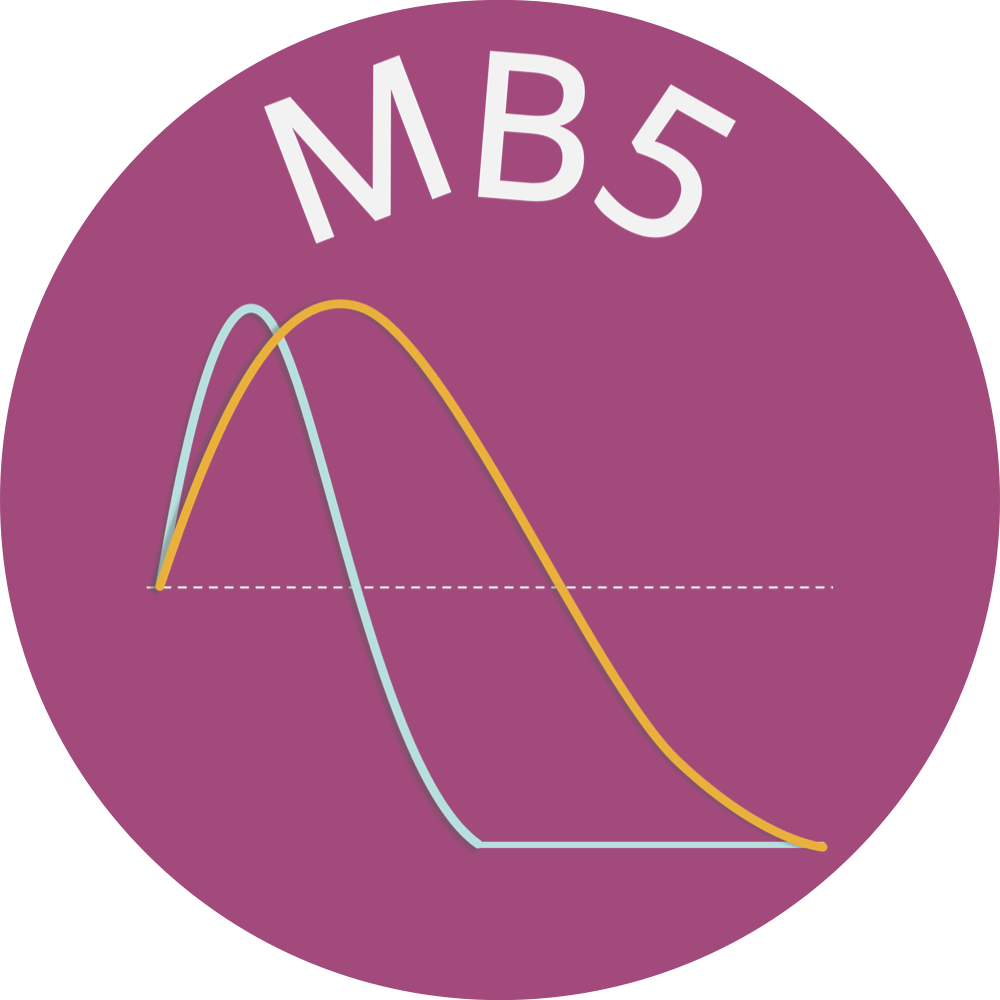
\includegraphics[width=0.3\textwidth,height=\textheight]{images/mb5-logo.png}

Thank you for contributing to \href{https://manybabies.org/MB5/}{\textbf{ManyBabies 5}} (MB5), a project of \href{https://manybabies.org/}{\textbf{ManyBabies}}, a cross-lab effort to provide an empirical basis for discussions of replicability as well as cultural, developmental, and methodological variability in infant perception/cognition research. In this project, we are examining drivers of infants' familiarity vs.~novelty preference through a collaboratively-designed ``best test'' of a popular model of infants' visual preference for familiar and novel stimuli \citep{hunterames}. More details about the background, design and hypotheses can be found in the \href{https://osf.io/preprints/psyarxiv/ck3vd}{\textbf{Registered Report}}. Below we provide instructions on how to implement the experiment in your lab and report data back to the project as a whole.

\hypertarget{mb5-project-website-manybabies.orgmb5}{%
\paragraph*{\texorpdfstring{\textbf{MB5 Project website:} \url{manybabies.org/MB5}}{MB5 Project website: manybabies.org/MB5}}\label{mb5-project-website-manybabies.orgmb5}}
\addcontentsline{toc}{paragraph}{\textbf{MB5 Project website:} \url{manybabies.org/MB5}}

\hypertarget{manybabies-general-manual-link}{%
\paragraph*{\texorpdfstring{\textbf{ManyBabies General Manual:} \href{https://docs.google.com/document/d/1dZ3sF2UcxvpkfOfKSKFeObTMZRbpUYloMUiPYtZy0ng/edit?usp=sharing}{link}}{ManyBabies General Manual: link}}\label{manybabies-general-manual-link}}
\addcontentsline{toc}{paragraph}{\textbf{ManyBabies General Manual:} \href{https://docs.google.com/document/d/1dZ3sF2UcxvpkfOfKSKFeObTMZRbpUYloMUiPYtZy0ng/edit?usp=sharing}{link}}

\hypertarget{mb5-collaboration-agreement-link}{%
\paragraph*{\texorpdfstring{\textbf{MB5 Collaboration Agreement:} \href{https://docs.google.com/document/d/1vbTDmH6euda5pJN4uyds3zsnQ1DXrW9wpHogwC-5TSk/edit?usp=sharing}{link}}{MB5 Collaboration Agreement: link}}\label{mb5-collaboration-agreement-link}}
\addcontentsline{toc}{paragraph}{\textbf{MB5 Collaboration Agreement:} \href{https://docs.google.com/document/d/1vbTDmH6euda5pJN4uyds3zsnQ1DXrW9wpHogwC-5TSk/edit?usp=sharing}{link}}

\hypertarget{mb5-stage-1-registered-report-kosiezettersten2024}{%
\paragraph*{\texorpdfstring{\textbf{MB5 Stage 1 Registered Report:} \citep{kosiezettersten2024}}{MB5 Stage 1 Registered Report: {[}@kosiezettersten2024{]}}}\label{mb5-stage-1-registered-report-kosiezettersten2024}}
\addcontentsline{toc}{paragraph}{\textbf{MB5 Stage 1 Registered Report:} \citep{kosiezettersten2024}}

\hypertarget{mb5-contact-mb5manybabies.org}{%
\paragraph*{\texorpdfstring{\textbf{MB5 Contact:} \url{mb5@manybabies.org} }{MB5 Contact: mb5@manybabies.org }}\label{mb5-contact-mb5manybabies.org}}
\addcontentsline{toc}{paragraph}{\textbf{MB5 Contact:} \url{mb5@manybabies.org} }

\begin{center}\rule{0.5\linewidth}{0.5pt}\end{center}

\hypertarget{lab-checklist}{%
\section*{Lab Checklist}\label{lab-checklist}}
\addcontentsline{toc}{section}{Lab Checklist}

\begin{enumerate}
\def\labelenumi{\arabic{enumi}.}
\tightlist
\item
  If you are new to MB5, complete the \href{https://docs.google.com/forms/d/e/1FAIpQLSdJnP3KO_dCmj-jNPHs0XP2j3q66g1RI6L31dwhCzhwhoJeoA/viewform}{Initial Sign-Up Form}.
\item
  Read this manual start to finish.
\end{enumerate}

\hypertarget{before-you-begin-data-collection}{%
\subsubsection*{BEFORE you begin data collection:}\label{before-you-begin-data-collection}}
\addcontentsline{toc}{subsubsection}{BEFORE you begin data collection:}

\begin{enumerate}
\def\labelenumi{\arabic{enumi}.}
\setcounter{enumi}{2}
\tightlist
\item
  Please ensure that you have carefully read the \href{https://docs.google.com/document/d/1vbTDmH6euda5pJN4uyds3zsnQ1DXrW9wpHogwC-5TSk/edit?usp=sharing}{MB5 Collaboration Agreement} and all of the documentation from the \href{https://docs.google.com/document/d/1dZ3sF2UcxvpkfOfKSKFeObTMZRbpUYloMUiPYtZy0ng/edit?usp=sharing}{ManyBabies General Manual} regarding \href{https://docs.google.com/document/d/1dZ3sF2UcxvpkfOfKSKFeObTMZRbpUYloMUiPYtZy0ng/edit\#heading=h.22i70rxou3ha}{ethical research}, \href{https://docs.google.com/document/d/1dZ3sF2UcxvpkfOfKSKFeObTMZRbpUYloMUiPYtZy0ng/edit\#heading=h.9ty2g48mpe0t}{authorship}, \href{https://docs.google.com/document/d/1dZ3sF2UcxvpkfOfKSKFeObTMZRbpUYloMUiPYtZy0ng/edit\#heading=h.aunbjkpwxhf3}{data sharing}, and \href{https://docs.google.com/document/d/1dZ3sF2UcxvpkfOfKSKFeObTMZRbpUYloMUiPYtZy0ng/edit\#heading=h.6h67zsyeiveg}{data use}.
\item
  Set up your study in consultation with this document. Carefully record any needed deviations from the protocol. Decide on your planned sample size/stopping rule.
\item
  Complete the Laboratory Questionnaire {[}insert link{]}, submit Ethics approval and other documentation/materials.
\item
  Create and submit your walkthrough video.
\item
  Run pilot sample through \href{https://manybabies.org/validator/}{data validator}.
\item
  Send email to \url{mb5@manybabies.org} to let the leadership team know that you are ready for `greenlighting'.
\item
  Wait for your official ``greenlight'' from the leadership team to begin data collection.
\end{enumerate}

\hypertarget{data-collection}{%
\subsubsection*{Data collection:}\label{data-collection}}
\addcontentsline{toc}{subsubsection}{Data collection:}

\hypertarget{important-do-not-begin-data-collection-other-than-piloting-until-you-have-been-explicitly-and-individually-greenlighted-to-do-so.}{%
\paragraph*{IMPORTANT: DO NOT begin data collection (other than piloting) until you have been explicitly (and individually) ``greenlighted'' to do so.}\label{important-do-not-begin-data-collection-other-than-piloting-until-you-have-been-explicitly-and-individually-greenlighted-to-do-so.}}
\addcontentsline{toc}{paragraph}{IMPORTANT: DO NOT begin data collection (other than piloting) until you have been explicitly (and individually) ``greenlighted'' to do so.}

\begin{enumerate}
\def\labelenumi{\arabic{enumi}.}
\setcounter{enumi}{9}
\tightlist
\item
  Collect your data!
\end{enumerate}

\hypertarget{after-you-finish-data-collection}{%
\subsubsection*{AFTER you finish data collection:}\label{after-you-finish-data-collection}}
\addcontentsline{toc}{subsubsection}{AFTER you finish data collection:}

\begin{enumerate}
\def\labelenumi{\arabic{enumi}.}
\setcounter{enumi}{10}
\tightlist
\item
  Complete your participant and trial data files in consultation with the data reporting instructions {[}insert link{]}.
\item
  Submit your data using the \href{https://docs.google.com/forms/d/e/1FAIpQLSdFYk-gb4yjRYLjSTP1_BVaW-3vLkpJClLoY2BOGDGfIVE5ww/viewform?usp=sf_link}{MB5 data upload form}.
\end{enumerate}

\begin{center}\rule{0.5\linewidth}{0.5pt}\end{center}

\hypertarget{getting-started}{%
\chapter{Getting Started}\label{getting-started}}

\hypertarget{start-and-end-date}{%
\section{Start and End Date}\label{start-and-end-date}}

Data collection officially started XXX and will initially run until XXX. Labs may join the MB5 project any time during the data collection period, provided that set-up and a formal ``green light'' is obtained, and data collection can be completed before the end date. However, we understand that there may be disruptions to data collection for various reasons. If you are having trouble meeting this timeframe, please alert the leadership team to discuss possibilities.

\hypertarget{ethics-approval}{%
\section{Ethics approval}\label{ethics-approval}}

It is a good idea to get started on your ethics approvals as soon as possible. Approvals must be in place and a copy submitted to the Drive folder (see below) before you can obtain a green light to collect data. Contact us \href{mailto:mb5@manybabies.org}{\nolinkurl{mb5@manybabies.org}} if you need advice on obtaining ethics approval.

MB5 and other ManyBabies projects ask labs to collect a number of \href{ADD\%20LINK\%20TO\%20PARTICIPANTS\%20SECTION}{demographic background variables} to be made public along with the main data, e.g.~parental education, sex, etcetera. Not all of those variables are part of the main analysis. Even so, it is highly relevant to collect them for follow-up and secondary analyses, and for checking the representativeness of the sample. Please contact us \href{mailto:mb5@manybabies.org}{\nolinkurl{mb5@manybabies.org}} if your ethics board raises concerns about collecting these data.

\hypertarget{please-make-sure-you-have-permission-to-publicly-share-anonymized-raw-data-including-required-demographic-info-as-this-is-a-condition-of-participation.}{%
\paragraph*{Please make sure you have permission to publicly share anonymized raw data (including required demographic info), as this is a condition of participation.}\label{please-make-sure-you-have-permission-to-publicly-share-anonymized-raw-data-including-required-demographic-info-as-this-is-a-condition-of-participation.}}
\addcontentsline{toc}{paragraph}{Please make sure you have permission to publicly share anonymized raw data (including required demographic info), as this is a condition of participation.}

\hypertarget{video-sharing}{%
\subsection{Video sharing}\label{video-sharing}}

We strongly encourage labs (where possible) to store/share video recordings of their testing on \href{https://nyu.databrary.org/}{Databrary}, which is a secure site for this purpose. You will need to ensure that you have ethics approval in place to do this, and collect specific consent for this purpose from your participants. In addition, you will become a member of Databrary, which will require approval from your institution, so it's helpful to start this process early. You can \href{https://nyu.databrary.org/user/register?page=create}{begin the registration process for Databrary here}. We are aware that many laboratories, particularly in the European Union, may not be allowed to use Databrary. In these circumstances we encourage labs to use alternative methods for sharing their videos where possible.

\hypertarget{upload-a-copy-of-your-ethics-approval-documentation}{%
\subsection{Upload a copy of your ethics approval documentation}\label{upload-a-copy-of-your-ethics-approval-documentation}}

Ethics documentation (e.g., IRB approval forms) should be submitted prior to data collection. Ethics forms should be uploaded using the \href{https://docs.google.com/forms/d/e/1FAIpQLScTTmcQl1P1F4UWe95Jo7u5bken40AyAefXCYUJ9iYbnWaG8Q/viewform?usp=sf_link}{MB5 Documentation Upload Form}. \textbf{Please ensure that all materials uploaded for ethics are clearly labeled in the filename with your LabID (e.g.~\emph{babylabPrinceton\_ethics.pdf}).} Check \href{https://manybabies.org/labids/}{here} for a complete list of LabIDs to confirm yours before uploading. In some cases, labs will already have approval for MB5 under an ``umbrella protocol'' (i.e., a protocol that covers multiple studies in one lab). In these cases, the ethics form should still be uploaded as described here.

\hypertarget{participants-and-recruitment}{%
\section{Participants and Recruitment}\label{participants-and-recruitment}}

\hypertarget{age-and-numbers}{%
\subsection{Age and numbers}\label{age-and-numbers}}

The minimum expected contribution is a full sample of 32 babies (preferred, if possible) or a half sample of 16 babies between 3 months, 0 days and 15 months, 0 days old.

\begin{itemize}
\tightlist
\item
  Try to distribute participant ages across the full range of ages if possible.

  \begin{itemize}
  \tightlist
  \item
    \textbf{Please report the exact age in days.} You can use an online tool such as: \url{https://www.calculator.net/age-calculator.html}
  \end{itemize}
\item
  In situations where labs planned but were unable to collect the minimum contribution, laboratory members will still be eligible for authorship. Alternative contributions may be requested by the Leadership Team in these circumstances.
\item
  A lab's sample size contribution \textbf{includes any infant who enters the laboratory}, even if they are eventually excluded (e.g., due to fussiness, experimenter error, etc).
\end{itemize}

While we encourage as much participation as you can spare, it is crucial to the success of the project that you treat our study with the same care as you would any other study in your lab with respect to recruitment procedures, timing of data collection, and RAs/RA training. Please do not commit to providing data to ManyBabies if this level of care is not possible.

\hypertarget{eligibility-and-exclusions}{%
\subsection{Eligibility and Exclusions}\label{eligibility-and-exclusions}}

\textbf{The only requirements for inclusion in MB5 are that an infants' age falls within the 3- to 15-month age range and that the infant has no known issues that would directly impede their ability to process visual stimuli.} Infants who are hard of hearing, premature, bilingual, etc can be included in the lab's sample.

Please determine participants' eligibility on the phone prior to scheduling them in the ManyBabies study to avoid testing ineligible participants, but note that the inclusion criteria for MB5 are much more inclusive than typical in-lab studies (described above). Participants who come into the lab who are subsequently determined to be ineligible should be reported in the sample.

\hypertarget{first-sessionsecond-session-policy}{%
\subsection{First-session/second-session policy}\label{first-sessionsecond-session-policy}}

Some laboratories have the practice of testing babies in more than one study during the same visit. \textbf{\emph{`First session'}} refers to babies tested soon upon arrival to the lab, prior to participating in any other studies. \textbf{\emph{`Second session'}} refers to any testing that is done after the first session.
* \textbf{Please contribute `first session' babies when possible.} It is possible that second session babies will contribute worse/weaker/different data with respect to the larger goals of determining effect sizes.
* \textbf{Please label `second session' babies} appropriately if infants were run in a different study on the same visit prior to their participation in MB5. Please also document the nature of the study run prior to MB5 for all `second session' participants (e.g., ``7 minute study of object categorization using eye-tracking'').

\hypertarget{setting-up-the-experiment}{%
\chapter{Setting up the experiment}\label{setting-up-the-experiment}}

\hypertarget{experiment-overview}{%
\section{Experiment Overview}\label{experiment-overview}}

Each baby will be presented with a series of 12 trials with one familiarization and two test phases each. During familiarization, a single stimulus is presented centrally on the screen. The test phase will consist of two stimuli, one familiar and one novel, presented side-by-side. The location of the stimuli will be switched in the two test trials. The duration of the familiarization will vary across trials (5, 10, or 15s). The tests will last 5s each. There will be two versions of the experiment: one in which the familiarization time will be pre-established (fixed-length), and another one in which the length of the trial will last until the infant accumulates the required looking time (infant-controlled).

\hypertarget{equipment}{%
\section{Equipment}\label{equipment}}

We assume you will use an experimental software (e.g.~Matlab, Habit, E-Prime, Psychopy, OpenSesame or custom software) to run the study and one of two settings to record looking times:
(1) Offline Video recording
(2) Eye-tracker (e.g.~Tobii, EyeLink, SMI, ASL, or a different company, with appropriate software from the eye-tracker or custom software).
(3) Eye-tracker + video recording
We also assume you know how to set up looking-time studies on your equipment. If that is not the case, or if you need help, support is available from the following people:
OpenSesame:
E-prime: Andreea Geambasu (\href{mailto:a.geambasu@hum.leidenuniv.nl}{\nolinkurl{a.geambasu@hum.leidenuniv.nl}})
PsychoPy: Silvia Benavides-Varela (\href{mailto:silvia.benavidesvarela@unipd.it}{\nolinkurl{silvia.benavidesvarela@unipd.it}}). (the psychopy experiment used by Silvia's group is here for other labs to use)
PyHab: Kateřina Chládková \href{mailto:chladkova@praha.psu.cas.cz}{\nolinkurl{chladkova@praha.psu.cas.cz}} or \href{mailto:Katerina.Chladkova@ff.cuni.cz}{\nolinkurl{Katerina.Chladkova@ff.cuni.cz}}

Eye tracking, using Tobii: Sylvain Sirois (\href{mailto:sylvain.sirois@uqtr.ca}{\nolinkurl{sylvain.sirois@uqtr.ca}})
Eye tracking, using SMI:
Eye tracking, using Eyelink: Julien Mayor (\href{mailto:julien.mayor@psykologi.uio.no}{\nolinkurl{julien.mayor@psykologi.uio.no}})
Other systems: email Casey Lew-Williams (\href{mailto:caseylw@princeton.edu}{\nolinkurl{caseylw@princeton.edu}}) and we'll do our best to help out.

\hypertarget{stimuli}{%
\section{Stimuli}\label{stimuli}}

All materials are available in our google drive folder.
Trial Structure. There are a total of 12 trials for each infant. Each trial will include both familiarization and test phases (described in further detail below). Between each trial, a laughing baby attention-getter will be presented.
Familiarization Trials. There are a total of 12 familiarization events for each infant that vary across three dimensions: (1) stimulus class (fractals or fribbles) ; (2) complexity level (low or high complexity); and (3) familiarization time (5s, 10s, or 15s); see table below. XXX
Infant-controlled Familiarization studies: If you are running the infant-controlled version of the study, infants may accumulate the required familiarization time across multiple exposures before advancing to the test trials.
Fixed Familiarization studies: If you are unable to collect infant-controlled accumulated looking for familiarization trials, then you will present the familiarization trials for a fixed length of time in one exposure before advancing to the test trial.
Stimulus Class
Complexity Level
Familiarization Time
Fribbles
Low Complexity
5 seconds
Fribbles
Low Complexity
10 seconds
Fribbles
Low Complexity
15 seconds
Fribbles
High Complexity
5 seconds
Fribbles
High Complexity
10 seconds
Fribbles
High Complexity
15 seconds
Fractals
Low Complexity
5 seconds
Fractals
Low Complexity
10 seconds
Fractals
Low Complexity
15 seconds
Fractals
High Complexity
5 seconds
Fractals
High Complexity
10 seconds
Fractals
High Complexity
15 seconds

Test Trials. Once the familiarization criterion has been reached, the infant will be presented with a central fixation stimulus and then paired test stimuli. Each pair of test stimuli includes the stimulus to which the infant was familiarized and a novel stimulus from the same stimulus class (fribbles or fractals) and complexity level (low-complexity or high-complexity). Infants will view the test stimuli for a total of 10s, separated into two phases. They will be presented with the familiar and novel stimulus for 5s after which a central fixation stimulus will be presented. The infant will then view the second 5s test phase, which uses the same two stimuli but with the location flipped (i.e., the image that was on the left in phase 1 will be on the right in phase 2).
Re-centering / Attention-getter stimulus
Between Trials. Please use the provided laughing baby stimulus to re-center babies between each trial (i.e., before familiarization begins).\\
Within Trial. Please use the provided attention-getter stimulus (the Hoehle circle with chimes) to re-center babies within each trial (i.e., between familiarization and test and between each of the test phases).
See below for a visualization of the trial structure:

\hypertarget{piloting-and-other-non-primary-data}{%
\section{Piloting and other non-primary data}\label{piloting-and-other-non-primary-data}}

Some labs might wish to pilot their design on a small number of infants in order to work out problems with the setup and allow experimenters to practice the protocol. Piloting with this purpose is indeed encouraged!
It is critical to the integrity of the ManyBabies project that these pilot data are carefully differentiated from your main contribution. You do NOT need to report pilot data in your spreadsheet, but if you do, please ensure that you properly mark them as such in the designated Pilot column.
You must make an explicit decision to begin non-pilot data collection at a particular date - this decision cannot be retroactive, and cannot be based on inspection of the pilot data (i.e., you cannot choose to include a pilot participant in the actual sample if the data ``looks good'').
Some labs might plan to test additional babies beyond the primary sample (e.g., with additional manipulations). These data will not be included in our primary planned analyses, and will not count toward the minimum contribution, but these additional datasets are welcome, and we encourage researchers to preregister other hypotheses. You are free to publish these ``side studies'' on your own terms, but please keep in mind the restrictions on publishing the main dataset if you are using it as a comparison/control sample (see the section on Open Science Policies in the MB General Manual).

\hypertarget{procedure}{%
\section{Procedure}\label{procedure}}

Please adhere to the following specifications for conducting this study. If any of the following technical specifications are not possible for your lab, please contact the MB5 leadership team (\href{mailto:mb5@manybabies.org}{\nolinkurl{mb5@manybabies.org}}) before beginning data collection to inform us of your planned deviation and the reason for it.

\hypertarget{caregiver-bias-and-instruction}{%
\subsection{Caregiver bias and instruction}\label{caregiver-bias-and-instruction}}

Caregivers should be masked from viewing the visual stimulus using your lab's standard method (e.g., having caregivers wear taped-over sunglasses).
It is not necessary to block parents' hearing of the audio stimulus.
Instruct parents NOT to point to the lights or screen, shift their bodies, or move their chairs if the baby is inattentive. Emphasize during the instruction/setup that infants' boredom with some of the stimuli is part of the experiment and is OK.
Suggestion: to ensure that the infant and parent are as comfortable as possible, you may tell the parent that it is okay to shift their or their baby's body to a more comfortable position, or provide interaction that the baby is soliciting, but emphasize that this may be done only for a short period during the attention grabber phase (e.g., when they hear the laughing baby).

\hypertarget{collecting-participant-information}{%
\subsection{Collecting participant information}\label{collecting-participant-information}}

We aim to integrate our testing procedure with your lab's procedure as much as possible, but there is some amount of information that we need to gather in a standardized fashion.
Participant information: Please use this Family Background Questionnaire to collect the information. You are welcome to adapt the format as long as the wording is not changed, except as noted:
Any areas marked in green you can adapt to ensure they are appropriate to your country/region. However, please keep the wording as similar as possible to ensure consistency in reporting.
The question on race/ethnicity can be adapted to meet the norms of your region. If possible, please use racial/ethnic categories taken from local census categories. For countries where it is not considered socially or legally acceptable to inquire about ethnic background, please adapt to a more appropriate question (e.g.~parent and child place of birth), if possible.
Translations into other languages will be available here as they are created.
If you need to make changes other than as indicated above, please contact the leadership team to discuss your concerns.
Let us know if any of the questions are unclear to you - it is important that you are able to answer any questions the participants may have. Please also check the participants' answers to avoid blank responses.
If you modify any of the wording in the form, even in the green sections, or translate the form to your lab's local language please upload a blank copy of your form using the MB5 documentation upload form. Please ensure that your form is clearly labeled in the filename with your LabID (e.g.~babylabPrinceton\_background.pdf).

\hypertarget{experimenter-blindness}{%
\subsection{Experimenter blindness}\label{experimenter-blindness}}

The experimenter should be masked fromblind to trial details, by being either (1) in a different room, with no way of knowing which stimuli the baby is seeing on each trial, or (2) in the same room but facing away from the stimuli and unaware of what is on the screen.

\hypertarget{sound-volume}{%
\subsection{Sound volume}\label{sound-volume}}

Your lab can use whatever volume level has been used successfully in the past, but please standardize your volume for this study so that every baby gets stimuli at the same volume.

\hypertarget{familiarization}{%
\subsection{Familiarization}\label{familiarization}}

Infant-Controlled Version (preferred version of data collection):
The visual stimulus is displayed until the infant accumulates 5, 10, or 15 seconds of looking (depending on familiarization condition). Infants' looking to the screen is tracked online in one of two ways: (1) automatically (e.g., using eye tracking methods); or (2) manually (e.g., experimenter presses a button while the infant is looking and releases when the infant looks away).
Fixed-Length/Duration Version:
The visual stimulus is displayed for 5, 10, or 15 seconds (depending on familiarization condition) regardless of the duration of infants' looking. Infants' looking to the screen may be measured offline (e.g., via later video coding) or online (e.g., experimenter presses a button while the infant is looking and releases when the infant looks away) to assess how much the infant actually looked to the stimulus during familiarization.

\hypertarget{test}{%
\subsection{Test}\label{test}}

Infant-Controlled Version (preferred version of data collection):
Circle \& chimes attention getter plays until the infant fixates for at least 500 ms total (can be accumulated across multiple looks).
After 500 ms is accumulated, the stimulus to which the infant was familiarized is presented alongside a novel stimulus (drawn from the same stimulus class (fribbles or fractals) and complexity level (low-complexity or high-complexity). The pair is presented for 5 s, regardless of how much the infant looks to the stimuli (i.e., duration of the test trials is fixed regardless of whether labs are using the infant-controlled or fixed-length version).
Circle \& chimes attention getter plays again until the infant fixates for at least 500 ms total (can be accumulated across multiple looks).
After 500 ms is accumulated, the same stimulus pair is presented for an additional 5s (regardless of how much the infant looks to the stimuli) with the side of familiar and novel stimulus reversed.
Infants' looking during test is calculated either: (1) automatically (if using an eyetracker); or (2) manually offline (e.g., coded from video data). Because it is challenging to manually code the side to which an infant is looking online, we request that labs who are not using an eyetracker code infants' looking during the test phase offline.
Fixed-Length/Duration Version:
Circle \& chimes attention getter plays for 750 ms (note that this is longer than the infant-controlled version to give infants time to fixate the central stimulus).
After 750 ms, the stimulus to which the infant was familiarized is presented alongside a novel stimulus (drawn from the same stimulus class (fribbles or fractals) and complexity level (low-complexity or high-complexity). The pair is presented for 5 s, regardless of how much the infant looks to the stimuli (i.e., duration of the test trials is fixed regardless of whether labs are using the infant-controlled or fixed-length version).
Circle \& chimes attention getter plays again for 750 ms.
After 750 ms, the same stimulus pair is presented for an additional 5s (regardless of how much the infant looks to the stimuli) with the side of familiar and novel stimulus reversed.
Infants' looking during test is calculated manually offline (e.g., coded from video data).

\hypertarget{general-lab-practices}{%
\section{General lab practices}\label{general-lab-practices}}

\hypertarget{training-research-assistants}{%
\subsection{Training research assistants}\label{training-research-assistants}}

You are responsible for implementing rigorous training practices. Research assistants should be held to the same high standards for ManyBabies as they would be for your main studies. You are free to have any number of research assistants conduct the test sessions, but please aim for as much coding consistency as possible and document which research assistant coded a given baby (using code names such as RA1, RA2, etc. if you wish). You will be asked to report about your standard training practices (e.g., how/when do you determine it's okay for a research assistant to test real babies).
Online Coding. If you are using a central screen to gather accumulated looking data for infant-controlled familiarization, then research assistants will need to be properly trained in coding online looking behaviors.
Offline Coding. If you are not using an eyetracker to gather data, then you will need to code the test trials offline.\\
Greeting families
You can greet families, briefly explain the study's purpose and goals in terms understandable to families (avoid technical jargon), obtain informed consent, and conduct the appointment as you normally would. Acknowledge their decision to consider participating and express appreciation for their time. Address potential concerns families might have and answer their questions openly and honestly.

\hypertarget{compensating-families}{%
\subsection{Compensating families}\label{compensating-families}}

You can use your lab's standard, IRB-approved method for compensating families. This can include providinge small gifts, cash, travel reimbursement, taxi rides, or other incentives for participation as you normally would. Participating labs are responsible for compensating their own participants.

\hypertarget{walkthrough-video}{%
\subsection{Walkthrough video}\label{walkthrough-video}}

Before beginning data collection, you are required to create a walkthrough video and submit it for approval. Instructions can be found here.
Upload your walkthrough video:
Walkthrough videos should be uploaded to this google drive folder. Please ensure that your video is clearly labeled in the filename with your LabID (e.g.~babylabPrinceton\_walkthrough.mpg).

\hypertarget{general-lab-practices-1}{%
\chapter{General Lab Practices}\label{general-lab-practices-1}}

\hypertarget{training-research-assistants-1}{%
\section{Training research assistants}\label{training-research-assistants-1}}

You are responsible for implementing rigorous training practices. Research assistants should be held to the same high standards for ManyBabies as they would be for your main studies. You are free to have any number of research assistants conduct the test sessions, but please aim for as much coding consistency as possible and document which research assistant coded a given baby (using code names such as RA1, RA2, etc. if you wish). You will be asked to report about your standard training practices (e.g., how/when do you determine it's okay for a research assistant to test real babies).
Online Coding. If you are using a central screen to gather accumulated looking data for infant-controlled familiarization, then research assistants will need to be properly trained in coding online looking behaviors.
Offline Coding. If you are not using an eyetracker to gather data, then you will need to code the test trials offline.

\hypertarget{greeting-families}{%
\section{Greeting families}\label{greeting-families}}

You can greet families, briefly explain the study's purpose and goals in terms understandable to families (avoid technical jargon), obtain informed consent, and conduct the appointment as you normally would. Acknowledge their decision to consider participating and express appreciation for their time. Address potential concerns families might have and answer their questions openly and honestly.

\hypertarget{compensating-families-1}{%
\section{Compensating families}\label{compensating-families-1}}

You can use your lab's standard, IRB-approved method for compensating families. This can include providinge small gifts, cash, travel reimbursement, taxi rides, or other incentives for participation as you normally would. Participating labs are responsible for compensating their own participants.

\hypertarget{walkthrough-video-1}{%
\section{Walkthrough video}\label{walkthrough-video-1}}

Before beginning data collection, you are required to create a walkthrough video and submit it for approval. Instructions can be found here.
Upload your walkthrough video:
Walkthrough videos should be uploaded to this google drive folder. Please ensure that your video is clearly labeled in the filename with your LabID (e.g.~babylabPrinceton\_walkthrough.mpg).

\hypertarget{prior-to-data-collection-checklist}{%
\chapter{Prior to data collection checklist}\label{prior-to-data-collection-checklist}}

The steps for getting started are tracked by the MB5 leadership team on the MB5 Project Tracker. You can check it to see what steps your lab has completed. If you have any questions or think your lab's progress is not up-to-date, contact us (\href{mailto:mb5@manybabies.org}{\nolinkurl{mb5@manybabies.org}}).

After preparing your lab and BEFORE BEGINNING DATA COLLECTION you need to:

\begin{itemize}
\tightlist
\item
  Complete the Initial Sign-Up Form (if you have not already done so).
\item
  Confirm ethics approval is uploaded: Make sure that a copy of your lab's ethics approval is in this google drive folder. If you plan to share participant videos via Databrary, you should also make sure you are getting proper consent for video sharing (please include approval for video sharing in ethics upload).
\item
  Confirm demographics form is uploaded: Make sure that a copy of your lab's demographics formethics approval is in this google drive folder.
\item
  Confirm walkthrough video is and demographics form uploaded (if needed): Make sure that a copy of your lab's walkthrough video is in this google drive folder, and your laboratory demographics form in this google drive folder.
\item
  Complete the Lab Questionnaire: Make sure someone from your lab has filled out the Lab Questionnaire with details about your laboratory. The leadership will be notified of your submission of the Lab Questionnaire after which they will start the approval/greenlighting process.
\item
  Convert dummy or pilot data into the right format for submission (see details below) using the MB Data validator to check data validity; in case of questions, please contact the analysis team. This ensures that you will be ready to submit your lab's data to the central analysis team!
\item
  Send email to Jessica Kosie (\href{mailto:jkosie@asu.edu}{\nolinkurl{jkosie@asu.edu}}) to let the leadership know that you are ready for `greenlighting'.
\item
  Wait until you receive an official go-ahead from Project Leads before you begin testing. We may have questions for you, e.g.~about your planned protocol deviations. We will do our best to respond quickly, but Iif you don't hear from us within a week of sending the email, please contact us again!.
\end{itemize}

\hypertarget{during-data-collection}{%
\chapter{During data collection}\label{during-data-collection}}

\hypertarget{equations}{%
\section{Equations}\label{equations}}

Here is an equation.

\begin{equation} 
  f\left(k\right) = \binom{n}{k} p^k\left(1-p\right)^{n-k}
  \label{eq:binom}
\end{equation}

You may refer to using \texttt{\textbackslash{}@ref(eq:binom)}, like see Equation \eqref{eq:binom}.

\hypertarget{theorems-and-proofs}{%
\section{Theorems and proofs}\label{theorems-and-proofs}}

Labeled theorems can be referenced in text using \texttt{\textbackslash{}@ref(thm:tri)}, for example, check out this smart theorem \ref{thm:tri}.

\begin{theorem}
\protect\hypertarget{thm:tri}{}\label{thm:tri}For a right triangle, if \(c\) denotes the \emph{length} of the hypotenuse
and \(a\) and \(b\) denote the lengths of the \textbf{other} two sides, we have
\[a^2 + b^2 = c^2\]
\end{theorem}

Read more here \url{https://bookdown.org/yihui/bookdown/markdown-extensions-by-bookdown.html}.

\hypertarget{callout-blocks}{%
\section{Callout blocks}\label{callout-blocks}}

The R Markdown Cookbook provides more help on how to use custom blocks to design your own callouts: \url{https://bookdown.org/yihui/rmarkdown-cookbook/custom-blocks.html}

\hypertarget{after-data-collection}{%
\chapter{After data collection}\label{after-data-collection}}

\hypertarget{publishing}{%
\section{Publishing}\label{publishing}}

HTML books can be published online, see: \url{https://bookdown.org/yihui/bookdown/publishing.html}

\hypertarget{pages}{%
\section{404 pages}\label{pages}}

By default, users will be directed to a 404 page if they try to access a webpage that cannot be found. If you'd like to customize your 404 page instead of using the default, you may add either a \texttt{\_404.Rmd} or \texttt{\_404.md} file to your project root and use code and/or Markdown syntax.

\hypertarget{metadata-for-sharing}{%
\section{Metadata for sharing}\label{metadata-for-sharing}}

Bookdown HTML books will provide HTML metadata for social sharing on platforms like Twitter, Facebook, and LinkedIn, using information you provide in the \texttt{index.Rmd} YAML. To setup, set the \texttt{url} for your book and the path to your \texttt{cover-image} file. Your book's \texttt{title} and \texttt{description} are also used.

This \texttt{gitbook} uses the same social sharing data across all chapters in your book- all links shared will look the same.

Specify your book's source repository on GitHub using the \texttt{edit} key under the configuration options in the \texttt{\_output.yml} file, which allows users to suggest an edit by linking to a chapter's source file.

Read more about the features of this output format here:

\url{https://pkgs.rstudio.com/bookdown/reference/gitbook.html}

Or use:

\begin{Shaded}
\begin{Highlighting}[]
\NormalTok{?bookdown}\SpecialCharTok{::}\NormalTok{gitbook}
\end{Highlighting}
\end{Shaded}

\hypertarget{additional-chapter}{%
\chapter{Additional Chapter}\label{additional-chapter}}

\hypertarget{heres-the-next-chapter}{%
\section{Here's the next chapter}\label{heres-the-next-chapter}}

Wow, really insightful!!

  \bibliography{refs.bib,packages.bib}

\end{document}
